\fancychapter{Experimental Methods}
\label{cap:Experimental-methods}

\textit{Over the experimental process, the appropriate settings of both the animals' state of alertness and of the visual stimulation were chosen as an operative practical balance. In this chapter we describe the methods and specifications of the animals' care and craniotomy cirurgies, as well as the settings of the ISOI and visual stimulation sessions.}

\section{Animals}
\label{sec:Animals}

All procedures were approved by the Champalimaud Centre for the Unknown Ethics Committee and carried under the stipulations of the Portuguese Direção Geral de Veterinária. Mice were held in individual cages on a reversed light-dark cycle with access to food and water. Mice were exclusively used for the experiments regarding this thesis' work.

Cells' somata in V1 layer 2/3 of four Thy1-GCaMP6s ?? male?? mice (?? Laboratory stock no:??) were imaged.

Prior to the imaging experiments, once adults (?? to ?? weaks old), the mice underwent chronic window implantation surgeries. A circular craniotomy of diameter $4mm$ was performed over each mouse's left visual cortex, leaving the dura intact. The imaging windows were constructed using two layers of microscope cover glass (Fisher Scientific, no. 1 and no. 2) and UV-curable optical glue. A window was placed into the craniotomy using black dental cement and an iron headpost was attached to the skull with dental acrylic. The subjects were kept under isoflurane anesthesia, as well as Bupivacaine ($0.05\%$; injected under the scalp) and Dolorex ($1 mg/kg$; injected subcutaneously), serving respectively as local and general analgesia. Eye moisturing was insured with ophtalmic ointment (Clorocil, Laboratorio Edol).

For both the ISOI and visual stimuli protocols, the animals were lightly anesthetized with isoflurane ($1\%$) and injected intramuscularly with chlorprothixene (1mg/kg), a muscular paralyzer to circumvert the need for higher anesthesia concentrations which could depress the recorded neuronal responses. Mice were headfixed by the headposts during all of the visual stimuli presentations and their eyes were protected and kept moist with silicone oil (Sigma-Aldrich) in thin, uniformly coated layers.

\section{Visual stimulation}
\label{sec:Visual-stimulation}

For both the ISOI and visual stimuli protocols, an LED display (BenQ XL2411Z, 144-Hz monitor, stimulus presented at $60 Hz$) was used. The screen was placed at $15 cm$ from the mouse's right eye and  aligned at $30º$ to the axis of its nose-line. The stimuli were produced and presented using Matlab and the Psychophysics Toolbox (see \ref{cap:TechnicalImplementations}. 

\section{Intrinsic signal optical imaging settings}
\label{sec:Intrinsic-signal-optical-imaging-settings}

The course of action with each craniotomized mouse started with the performance of intrinsic signal optical imaging (ISOI) over the mice's primary visual cortex and surrounding visual areas to obtain a reasonable spatial resolution retinotopic mapping of the temporaly dependent hemodynamics of the accessed brain while moving visual stimuli was presented to the animal on a monitor aligned to the center of the mouse's right eye and forming a $30º$ angle with the animal's nose-line.

The stimuli consisted of a checkerboard of alternate flickering light/dark squares ($5 Hz$) that was masked to continuously expose only a periodic drifting stripe of the grid in four consecutive cardinal directions ($12 s$ period, $20º$ width, 80 times for each direction) - an horizontal stripe going from the top to the bottom of the screen, vice-versa, a vertical stripe going from its left to its right or in the opposite direction.

The cortical surface of an head-fixed mouse was illuminated with a $620 nm$ red LED to allow the intrinsic hemodynamic signals to be recorded as optical images of reflectance change correspondent to cortical activity. This recording was held using a Retiga QIClick camera (QImaging) controlled with Ephus with a high magnification zoom lens (Thorlabs) at $5 Hz$ focused under the cranial window, at the brain surface. A $535 nm$ green LED was also used to obtain an image of the cortical vasculature.

For each animal, this resulted in a retinotopical map of $512 \times 512$ pixels, representing $400 \times 400$ of cortical area. This corresponded to the color-map of cortical encoding of both azimuth and elevation stimuli locations, superimposed on the image of the mouse's vasculature (images \ref{vessels} and \ref{mapping}). These correspondence figures were subsequently used as a first-approach guide to encountering the V1 positions aimed for imaging - those whose neurons responded to stimuli in the center of the mouse's visual field where the central stimuli were displayed during the following two-photon microscopy imaging sessions.
\begin{figure}[H] \centering 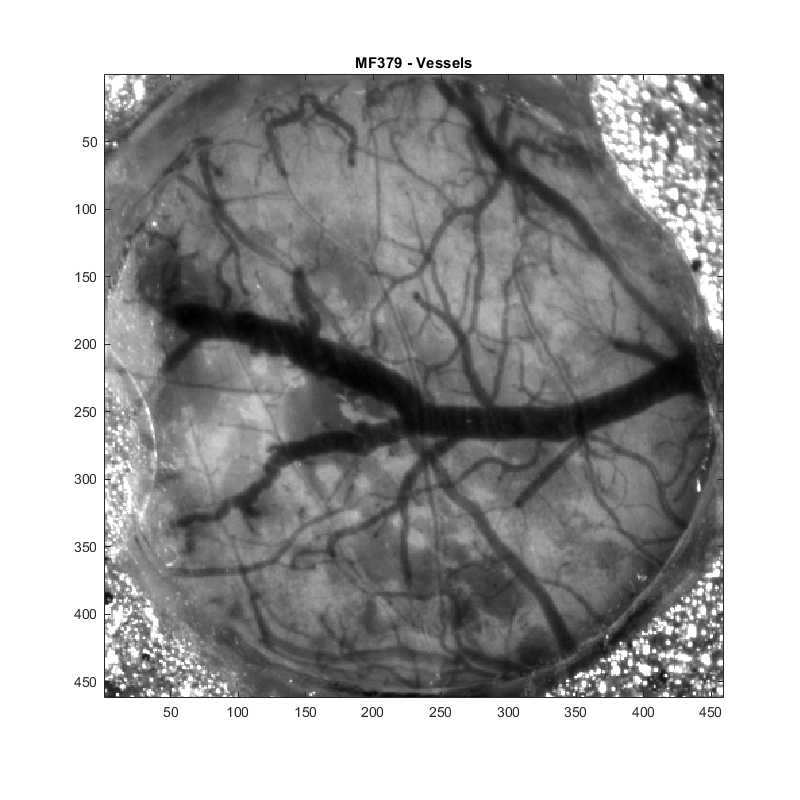
\includegraphics[width=7cm,height=7cm,keepaspectratio]{Figures/7.Results/intrinsic/MF379_Vessels.png} 
\caption{Vessels image obtained with ISOI for an example animal.}
\label{vessels}
\end{figure}
\begin{figure}[H] \centering 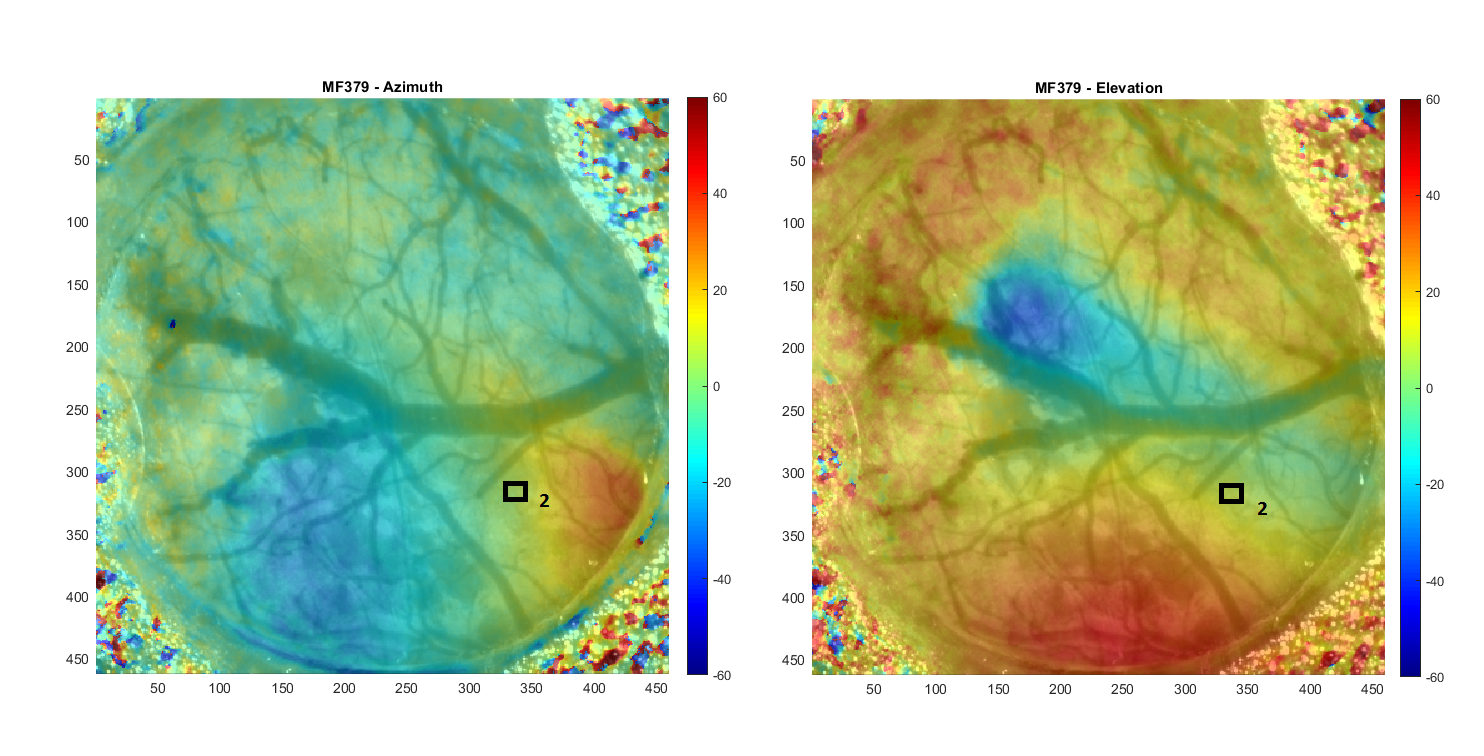
\includegraphics[width=13cm,height=13cm,keepaspectratio]{Figures/7.Results/intrinsic/mapping.png} 
\caption{ISOI azimuth and elevation maps for an example animal.}
\label{mapping}
\end{figure}

%\subsection{Subsection A}
%\label{subsec:subasectionA}
\section{Session and trial structure}
\label{sec:Session-and-trial-structure}

\subsection{TPLSM experimental pipeline}

An imaging session followed the same process in each experiment, starting with the setting up of a rig.
As a first step, the laser was turned on from its standby mode, about 30 minutes before conducting the scanning. This was the required time for the device to warm up to consistent power levels.

Besides the laser, the objective's motor, connected to the two-photon computer, was also turned on, as well as the heating pad to place the animal on and keep its thermal balance whilst anaesthetized. The laser's shutter was also opened as well as the pockel cells that control the light delivered to the animal's brain. Furthermore, the laser source was shared between two rigs, which meant that at each session one should confirm that the mirrors were rotated to the appropriate angle to send light to the rig being used. Furthermore, the system had two operation modes that could be interchanged with a switcher: Full brightness and two-photon imaging modes. With the PMT off, the experiment was to start with the switch to full brightness mode.

During this time, both the stimuli computer and the two-photon computer were turned on, and the rig was wired to bpod mode. In the stimuli computer, two matlab instances were opened, one for bpod states machine and GUI and another for psychtoolbox's stimuli presentation. In the two-photon computer, Bonsai light contamination control system was put to play, and a matlab instance was opened to start scanImage 4 laser-scanning software control system.

The animal to be imaged was manually removed from its cage and placed in a box to be anaesthetized with isoflurane, initially at $3.5\%$, delivered by a ventilation tube, mixed with oxygen at pressure of $1 atm$. Once the animal was unconscious, the paralyser chlorprothixene ($1 mg/kg$) was injected intramuscularly, and the animal was put back in the anaesthetizing box. At this point, the isoflurane ventilation was switched from the box to the rig's tube and the animal was quickly and carefully moved from the box to a platform in the rig under the objective, over the heating pad, confirmed to be at $34ºC$, with a mouth piece connected to the anaesthesia tube surrounding its fur. The mouse's headpiece was then locked to fixation screws and the animal's eyes were protected with an uniform layer of eye ointment; the anaesthesia was then set to a $1\%$ value, maintained during the rest of the session.

The cranial window was cleaned with deionized water as well as the objective, with the aid of Thorlab paper for optical components. A black plastic ring was then glued to the cranial window, in order to minimize contamination of the collected fluorescence signals with monitor light. Imaging gel was placed over the cranial window, with care for not keeping air bubbles that could impeach the light path, and for keeping full uniform contact between the gel and the imaging window.

The imaging system was initially in full brightness mode with the PMT turned off. Camera software was then opened and configured in the two-photon computer, to aid with full-brightness mode navigation. With this, a pedal enabled a green light to be sent from the objective, aiding in the alignment of the animal's cranial window within the full range of the objective's motor: the animal's platform was moved to the appropriate objective-aligned placing and the objective was then moved down in depth until reaching the gel and until the software displayed visible blood vessels.
The stimuli presentation monitor was then centred to the animal's right eye gaze, at $15 cm$ from his eye and at a $30º$ angle with its body's axis. Finally, a light shield was placed over the objective and the rubber ring in the animal's cranial window, ensuring good blockage of the monitor's contamination light to the signal's light path. The room's lights were filtered for only passing red light and the rig was then closed with a black cloth to further seclude it from light contamination and PMT damage. 

With the intrinsic azimuth and elevation maps rotated to match the objective's signal display on the camera software, with the green light on, one would then search for the (0,0) corresponding position in V1, using the larger blood vessels as guidelines. Having found this placing, the pedal was left off, and the PMT could be turned on for two-photon mode imaging with the ScanImage software.

The configurations in ScanImage were set to multiplane scanning (5 planes). The laser was calibrated, and the voltage - angle calibration curve was confirmed linear. Bpod was started with a Tuning protocol, with a small-sized circular center grating stimuli being presented in multiple directions and frequencies, to further aid in searching for V1 (0,0) position. Bpod setting's were submitted, and psychtoolbox protocol could be initiated, preparing the stimuli.

The scanning could be started with ScanImage GUI set to expect no external triggering, for continuous signal collection through time. The green channel's signal for each imaged plane could then be seen, in ScanImage GUI. Going down in depth, one starts to detect the dura of the brain. At this point, the motor coordinates should be set to zero. 
In these experiment, one would go further down to $150 \mu m$ to $210 \mu m$ center plane depth, until neurons could be detected.

Once the stimuli masks were ready, the \textit{Start} button in bpod's GUI initiated the stimuli presentation. With this small centred stimuli being displayed to the mouse, one could then search for the close positions in the mouse's brain that were more strongly responding with locked timings to the stimuli presentation. 

Having found this position, the recordings were started, fixed to external triggering coming from bpod's device. A reference image was print screened and kept for checking and managing possible drift of the imaging planes during the session, due to cranial window or brain micro movements. During the session, one should also keep checking the trial number synchronization between scan image recordings, psychtoolbox presentation and bpod triggers, in both computer GUIs.

\subsection{Stimuli presentation structure}

The experimental recorded stimuli presentation of a session comprised three main protocols for each mouse and each of that animal's V1 imaged position: A protocol to establish the receptive fields of the imaged neurons ($\texttt{StimPresProt\_RF}$), another to regard their tuning properties ($\texttt{StimPresProt\_tuning}$) and a last protocol designed for the actual surround modulation examinations ($\texttt{StimPresProt\_RF}$). 

Each protocol involved a pseudorandomized sequence of trials - N repetitions of X trial types. Repetitions of each stimulus type are required in order to enhance the signal to noise ratio of the responses by trial averaging. 

In general, each trial was formed by an initial baseline, a stimulus presentation, and an inter-trial interval (ITI). In both the baseline and the ITI the screen was left at background brightness and contrast level (grey) and its duration was used as buffer time for internal computations and to ensure sufficient Calcium decay from the previous stimulation (from the previous trial in the case of the baseline, and from the same trial in the case of the ITI). A session's total stimuli display duration should not be longer than two hours, as the anesthesia produces cumulative effects in the central nervous system and can start depressing the neuronal responses, impeaching the subsequent study of its relation with the visual stimulation [REFERENCES]. Thus, the durations of these intervals depended on the specific protocol (chapter 4, section d), as a balance between how important was the separation of responses in between trials - the more precise the intended separation, the larger should be the baseline and ITI durations - and how many trial types and trial repetitions were intended - the more trials, the less duration the baseline and ITI should have.

 \begin{table}[H]
\begin{center}\par
\scalebox{0.85}{
\begin{tabular}{c|cccccccccccccccccccccccccc}
\hline 
 
    
           & \multicolumn{ 1}{c}{Number of trial types} & Number of repetitions &     baseline (ms) & stimulus (ms)& ITI (ms) \\
           
           \hline
           \hline

RF & 80 & 14 & 0 & 880 & 120 \\
tuning & 32 & 25 & 5 & 900 & 95 \\
SM & 124 & 15-20 & 500 & 1000 & 500 \\

\hline
        
\end{tabular}}
 \caption{Protocol configurations regarding session extension and trial durations.}
    \vspace{-5mm}
    \label{table:times}
\end{center}
\end{table}
\section{Specifics of the protocol settings and visual stimuli}
\label{sec:Specifics-of-the-protocol-settings-and-visual-stimuli}

In a session, the three stimuli presentation protocols were ordered as RF mapping, tuning mapping and then the actual SM examination.
Each protocol is associated with different stimuli characteristics, specific to the controls or information that were to be required from the final extracted data. Furthermore, each kind of protocol had also distinct specifications in regards to the time durations in the trial structure of the session.
The mice were always placed with their right eye parallel and at $15 cm$ from the center of the monitor. All of the stimuli measurements will thus follow indicated in degrees at the mice's perspective to the screen, in azimuth (horizontal axis) and in elevation (vertical axis) coordinates. In addition, to compensate for the screen's flatness, spherical corrections were applied to the displayed stimuli, so that what the mice visualized corresponded to the same size of stimuli at each patch location, irrespective of its distance in the screen and that no distortions in the gratings were perceived by the animal.
Every protocol underwent pseudorandomization of the trials: Each type of trial appeared the same number of N repetitions, but at shuffled order. The reason for this was to minimize the neurons adaptation [REFERENCES] to the specific trial types, as they had to be repeated a reasonable amount of times for significant analysis.

\subsection{Receptive Field mapping stimuli}
\label{subsec:subasectionC}

This protocol consisted on the presentation of a 10º squared cell (in the mouse's referential) with a small moving bar inside. At each trial, this bar moved in four directions, in sequence but at random order - bottom to top (labelled 0º), left to right (90º) and the opposite ones (180º and 270º, respectively). The moving bar had $4º$ width and $25 º/s$ speed, with the dark at $0 WHAT$, the light at $204 WHAT$ and the background at $102 WHAT$. This patch appeared in any of 80 positions in the monitor, which was divided in a $10 \times 10$ grid, tiling a circle with 50º maximum radius from the center. The presentation was repeated in each grid position 14 times, to a total of 1120 trials, at shuffled order whithin each repetition.

At each trial of $1 s$, the stimulus played for $220 ms$ and was followed by an $880ms$ ITI, summing 19 minutes of RF mapping at each session. 

 \begin{table}[H]
\begin{center}\par
\scalebox{0.85}{
\begin{tabular}{c|cccccccccccccccccccccccccc}
\hline 
 
    
\multicolumn{1}{c}{Feature} & Value \\
           
           \hline
           \hline

\multicolumn{1}{c}{cell size (º)} & 10 \\
\multicolumn{1}{c}{cell grid (º)} & [10, 10] \\
\multicolumn{1}{c}{maximum radius (º)} & 50 \\
\multicolumn{1}{c}{stim directions (º)} & [0 90 180 270] \\
\multicolumn{1}{c}{bar width (º)} & 4 \\
\multicolumn{1}{c}{bar speed (º/s)}& 10 \\
\multicolumn{1}{c}{dark, stim, background light} & [0 204 102] \\
\hline
        
\end{tabular}}
 \caption{Configurations regarding the RF mapping protocol stimuli properties.}
    \vspace{-5mm}
    \label{table:RF}
\end{center}
\end{table}

\begin{figure}[H] \centering 
\includegraphics[width=10cm,height=10cm,keepaspectratio]{Figures/4.Chapter/rf.png} \caption{rf example.} \end{figure}

\subsection{Tunings mapping stimuli}
\label{subsec:subbsectionC}

The selectivity of each neuron was also controlled for spatial and temporal frequencies, as well as for more gratings' directions of movement. 

With the same contrast configurations as for the previous protocol, a circular centered patch of $30º$ was presented at any of 8 directions: the previous and the intermediatedly oriented ones ($0º$, $45º$, $90º$, $135º$, $180º$, $225º$, $270º$ and $315º$). The gratings could have $0.02 /º$ or $0.04 /º$ of spatial frequency and $0.5 Hz$ or $1 Hz$ as temporal frequency. Together, each of these 32 configurations of direction and frequencies were presented in 25 repetitions, totaled at 800 trials and shuffled within the full protocol.

Each trial had $1 s$, divided in a baseline of $5 ms$, a stimulus presentation of $900 ms$ and an ITI of $95 ms$, to a total of 14 minutes per session.

\begin{table}[H]
\begin{center}\par
\scalebox{0.85}{
\begin{tabular}{c|cccccccccccccccccccccccccc}
\hline 
 
    
\multicolumn{1}{c}{Feature} & Value \\
           
           \hline
           \hline

\multicolumn{1}{c}{stimulus size (º)} & 30 \\
\multicolumn{1}{c}{stimulus center (º)} & [0, 0] \\
\multicolumn{1}{c}{stim directions (º)} & [0 45 90 135 180 225 270 315] \\
\multicolumn{1}{c}{spatial frequency (/º)} & [0.02 0.04] \\
\multicolumn{1}{c}{temporal frequency (Hz)}& [0.5 1] \\
\multicolumn{1}{c}{dark, stim, background light} & [0 204 102] \\
\hline
        
\end{tabular}}
 \caption{Configurations regarding the tuning mapping protocol stimuli properties.}
    \vspace{-5mm}
    \label{table:tuning}
\end{center}
\end{table}

\begin{figure}[H] \centering 
\includegraphics[width=4cm,height=4cm,keepaspectratio]{Figures/4.Chapter/tuning.png} \caption{tuning example.} \end{figure}

\subsection{Surround Modulation stimuli}
\label{subsec:subcsectionC}

Finally, for the SM protocol the frequencies of $0.04 /º$ and $1 s$ were chosen based on previous reports of largest V1 stimulation [REFERENCES]. The light contrasts of the gratings went from $0$ at dark to $122.5$ at background and $255$ at the lightest. Each trial had $2 s$, with $0.5 s$ of baseline, $1 s$ of stimuli display and $0.5 s$ of ITI. 

There were 124 possible trial types, repeated 20 times, to a total of 2480 trials in an 1 hour and 23 minutes session.

 \begin{table}[H]
\begin{center}\par
\scalebox{0.85}{
\begin{tabular}{c|cccccccccccccccccccccccccc}
\hline 
 
    
\multicolumn{1}{c}{Feature} & Value \\
           
           \hline
           \hline

\multicolumn{1}{c}{spatial frequency (/º)} & 0.04 \\
\multicolumn{1}{c}{temporal frequency (Hz)} & 1 \\

\multicolumn{1}{c}{central radius (º)} & 15 \\
\multicolumn{1}{c}{surround inner and outer radius (º)} & [27 50] \\
\multicolumn{1}{c}{stim directions (º)} & [0 90 180 270] \\
\multicolumn{1}{c}{dark, stim, background light} & [0 255 122.5] \\
\multicolumn{1}{c}{groups of stimuli} & C, S1, S1+C, S2, S2+C \\
\hline
        
\end{tabular}}
 \caption{Configurations regarding the SM protocol stimuli properties.}
    \vspace{-5mm}
    \label{table:SM}
\end{center}
\end{table}

There were 5 possible patches: a central one and four surround patches in the cardinal positions. The central patch was a circle of 15º radius, as the others were limited by an external circumference of 50º, an inner circumference of 27º (to obtain a 12º gap between the center and the surround patches) and the curresponding bissectors of the screen. For any patch, there were 4 available directions of gratings movement ($0º$, $90º$, $180º$ and $270º$).

With these patches, five groups of stimuli types were used:
\begin{itemize}
\item $C$ - only the center patch, in any of the 4 directions of movement (4 types);

\begin{figure}[h]\centering 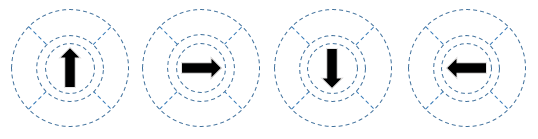
\includegraphics[width=9cm,height=9cm,keepaspectratio]{Figures/4.Chapter/C.PNG} \caption{Diagram of stimuli group C.} \end{figure}

\item $S1$ - only one surround patch, in any of the 4 cardinal top, bottom, left or right locations (S1T, S1B, S1L, S1R), and in any of the 4 directions (16 types);

\begin{figure}[h]\centering 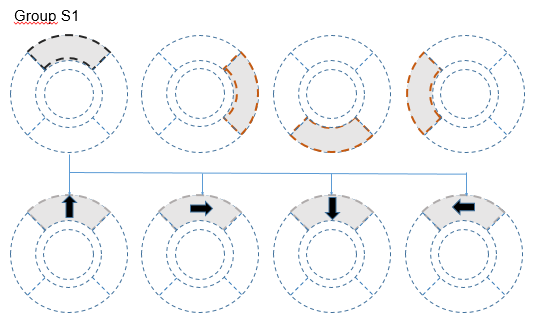
\includegraphics[width=9cm,height=9cm,keepaspectratio]{Figures/4.Chapter/S1.PNG} \caption{Diagram of stimuli group S1.} \end{figure}

\item $S1+C$ - One surround patch and the center patch, at any location of the surround($S1T+C$, $S1B+C$, $S1L+C$, $S1R+C$) and any direction for the center and for the surround (64 types);

\begin{figure}[H] \centering 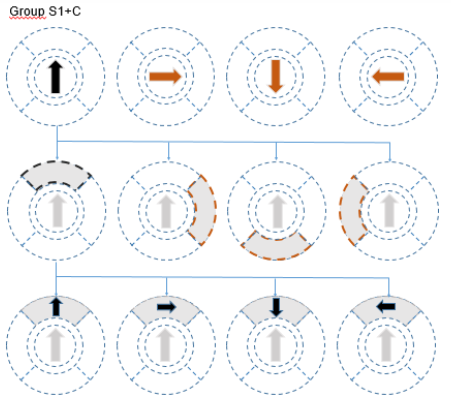
\includegraphics[width=9cm,height=9cm,keepaspectratio]{Figures/4.Chapter/S1C.PNG} \caption{Diagram of stimuli group S1C.} \end{figure}

\item $S2$ - only two surround patches, in opposite cardinal locations, either in the horizontal line ($S2H$) or the vertical line ($S2V$), both of them with gratings moving in the same of any of the 4 directions (8 types);

\begin{figure}[H] \centering 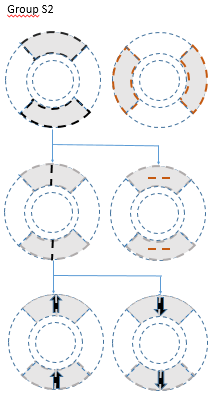
\includegraphics[width=8cm,height=8cm,keepaspectratio]{Figures/4.Chapter/S2.PNG} \caption{Diagram of stimuli group S2.} \end{figure}

\item $S2+C$ - Two surround patches and the center patch, both surround patches either in the horizontal ($S2H+C$) or the vertical line ($S2V+C$), both with gratings moving in the same of the possible directions and the center patch with gratings moving in any direction, not necessarily being the same from the surround stimuli (32 types).

\begin{figure}[H] \centering 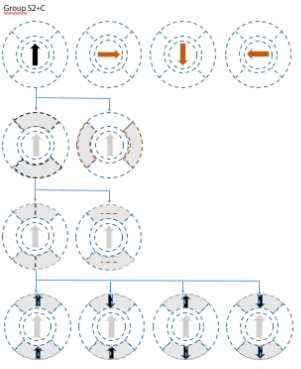
\includegraphics[width=10cm,height=10cm,keepaspectratio]{Figures/4.Chapter/S2C.PNG} \caption{Diagram of stimuli group S2C.} \end{figure}

\end{itemize}


\begin{figure}[H] \centering 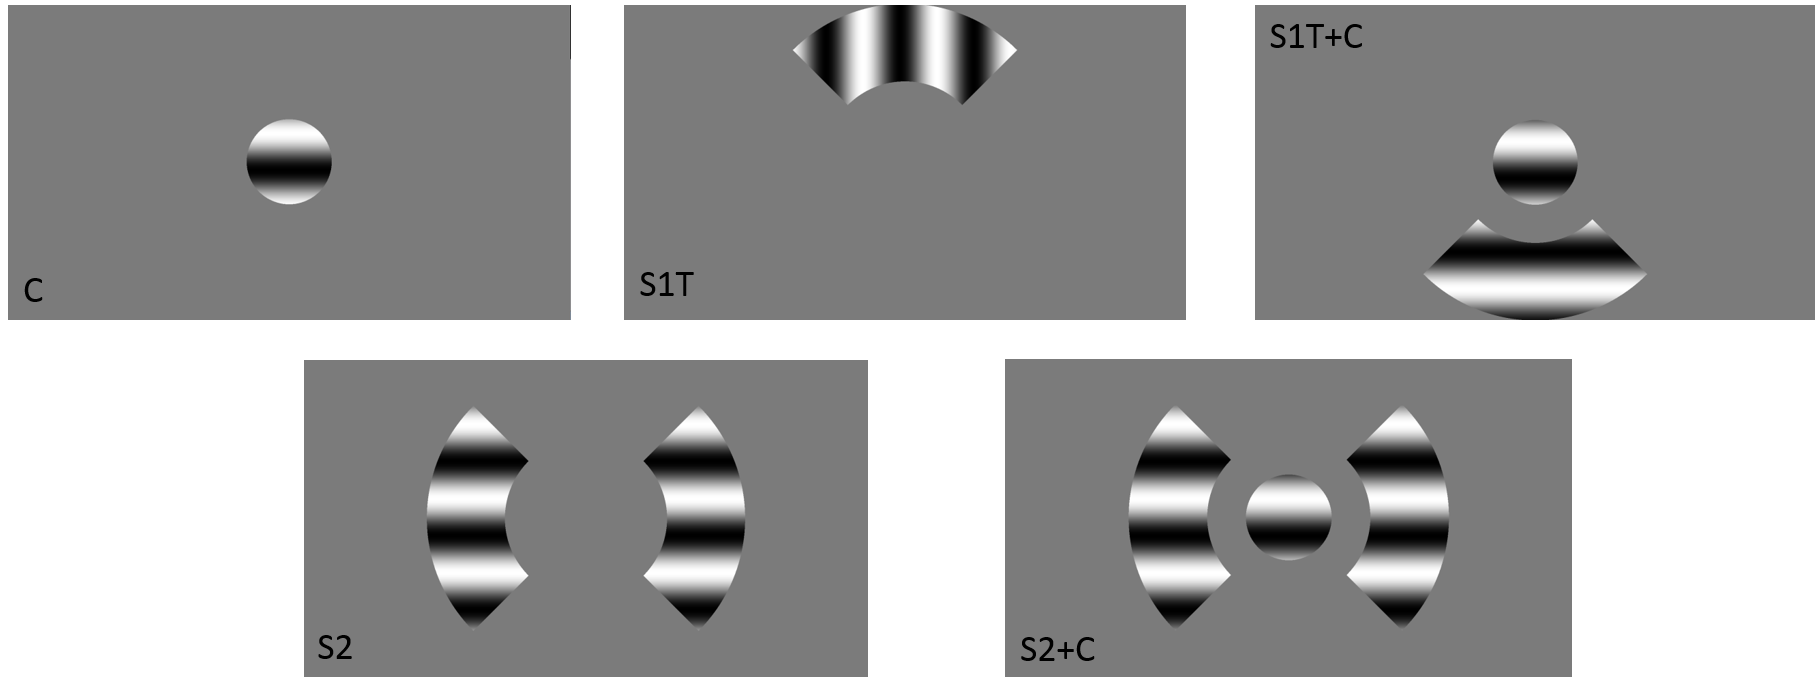
\includegraphics[width=12cm,height=12cm,keepaspectratio]{Figures/4.Chapter/SM.png} \caption{SM examples.} \end{figure}

Group $C$ was used as a more specific confirmation for the receptive field findings: here the stimuli was now in the center of the screen with the selected size for the analysis. Groups $S1$ and $S2$ provided the data that allowed to exclude from the analysis the cells that responded to stimulation in the defined surround. These had a receptive field that overlapped what we regarded as the surround and thus did not meet the criteria for investigating surround modulation effects in this experiment's designed manner. With the cells that did respond to group $C$ but did not to group $S1$ nor $S2$, we could then regard the effects of actual surround stimulation by examinating the responses to stimuli in the groups $S1+C$ and $S2+C$.
\cleardoublepage